  \chapter{Introdução}
  
  \section{Motivação}
  %Escrever sobre o cenário de software propício para chatbots. Falar sobre chatbots vs apps e uso das redes sociais.
  As redes sociais tem o papel de conectar pessoas, estreitando assim os laços humanos. Graças a elas podemos nos comunicar com pessoas que estão do outro lado do globo em tempo real. O sucesso das redes sociais é tão grande, que apenas no Brasil, temos cerca de 130 milhões de usuários mensais só no Facebook. Segundo dados da pesquisa 143ª Pesquisa CNT/MDA\footnote{https://www.cnt.org.br/agencia-cnt/confira-resultados-pesquisa-cnt-mda}, 82\% dos entrevistados afirmam que fazem uso de seus \emph{smartphones} para acesso à redes sociais. Além disso, os resultados da 29ª Pesquisa Anual de Administração e Uso de Tecnologia da Informação nas Empresas, realizada pela FGV, mostra que o Brasil já ultrapassou a marca de 1 aparelho \emph{smartphones} por habitante\footnote{https://eaesp.fgv.br/sites/eaesp.fgv.br/files/pesti2018gvciappt.pdf}.
  
  O tamanho sucesso das redes sociais e dos \emph{smartphones}, permitiu que os antigos sistemas de informação, que, em algumas décadas atrás necessitavam de grandes computadores para serem executados, agora são acessíveis por um dispositivo de mão. Jogos, bancos, redes sociais, e até mesmo redes de \emph{fast-food} desenvolveram seus aplicativos e marcaram presença nos \emph{smartphones} da população. Estima-se que apenas na Play Store (loja de aplicativos do Google), cerca de 2,6 milhões de aplicativos estejam disponíveis para \emph{download}\footnote{https://www.statista.com/statistics/266210/number-of-available-applications-in-the-google-play-store/}.
  
  Contudo, estudos mais recentes indicam que apenas cinco aplicativos são responsáveis por cerca de 84\% do uso de de aplicativos não nativos do smartphone\footnote{https://techcrunch.com/2015/06/22/consumers-spend-85-of-time-on-smartphones-in-apps-but-only-5-apps-see-heavy-use/}. Esses aplicativos variam de pessoa para pessoa, mas em geral, incluem aplicativos de redes sociais ou de mensagens instantâneas. Esse cenário justifica o aumento no número de chatbots disponíveis em plataformas de mensagens como Messenger nos últimos anos.
  
  % definir o que é chatbot %
  \textit{Chatbots} são sistemas computacionais que simulam uma conversas com pessoas e tornam a interação homem-máquina mais natural\cite{chatbot_definition}. São comumente chamados de assistentes virtuais, agentes virtuais ou simplesmente \textit{bots}.
  % / definir o que é chatbot %
  
  Ao criar um \emph{chatbot} para ser utilizado em canais já consolidados como Messenger, Telegram, Slack e WhatsApp, estamos utilizando uma infraestrutura já consolidada de um aplicativo para executar tarefas que um usuário faria em um outro aplicativo, o que dispensa a instalação e ocupação da memória do aparelho do usuário. Além disso, \textit{chatbots} também podem ser incluídos em \textit{sites} oferecendo aos visitantes um canal rápido de atendimento enquanto navega na internet.
  
  Outro ponto é que o formato de comunicação através de troca de mensagens oferecido pelos \emph{chatbots} é mais humano do que a interação em um aplicativo convencional. O usuário tem uma dúvida e, ao invés de navegar entre menus e telas de um aplicativo, ele simplesmente envia seu questionamento e é prontamente respondido pelo \textit{bot}.
  
  Do ponto de vista de quem oferece a aplicação, ter um \emph{chatbot} ao invés de um aplicativo significa não ter que competir para captar usuários em uma loja de aplicativos, que por sua vez é repleta de outros aplicativos que são potenciais concorrentes.  Além disso, o custo de desenvolvimento tende a ser inferior, o que também é uma vantagem. Ao criar um \emph{chatbot}, criamos um único serviço que poderá estar disponível em um ou mais canais de comunicação, utilizando a mesma estrutura. Quando criamos aplicativos, especialmente aqueles que estarão disponíveis em várias plataformas, gastamos tempo pensando na experiência do usuário para dois ou mais sistemas diferentes e, por fim desenvolvendo dois aplicativos com estruturas diferentes.
  
  
  
  
  % https://br.newsroom.fb.com/company-info/
  
  % https://www1.folha.uol.com.br/tec/2018/07/facebook-chega-a-127-milhoes-de-usuarios-mensais-no-brasil.shtml
  
  % https://exame.abril.com.br/negocios/dino/62-da-populacao-brasileira-esta-ativa-nas-redes-sociais/
  
  % https://www.cnt.org.br/agencia-cnt/confira-resultados-pesquisa-cnt-mda
  
  % https://eaesp.fgv.br/sites/eaesp.fgv.br/files/pesti2018gvciappt.pdf
  
  % https://techcrunch.com/2015/06/22/consumers-spend-85-of-time-on-smartphones-in-apps-but-only-5-apps-see-heavy-use/
  
  % Avaliar um chatbot --------- https://www.forbes.com/sites/forbesagencycouncil/2018/06/04/using-facebook-messenger-and-chatbots-to-grow-your-audience/#760a4a8733b1
  
  \section{Objetivos}
  % O que se espera ter como produto final?
  % - O objetivo é construir o chatbot tendo como base boas práticas de ES.
  % Que portal? Você não disse que teremos duas versões do bot, etc. 
  
  O objetivo principal desse trabalho é construir um \textit{chatbot} tendo como base boas práticas de engenharia de software. O \textit{bot} deverá ser disponibilizado em duas plataformas: \textit{web}, para ser incorporado ao Portal do PIPA (site institucional do projeto, onde os pacientes cadastrados podem consultar informações e exames) e \textit{Messenger}. No que diz respeito a funcionalidades, ele deverá ser capaz de dar informações sobre o projeto para o público geral e poderá acessar os usuários cadastrados no portal PIPA, podendo vincular um paciente ao usuário do \textit{bot}. Aos pacientes que realizaram esse vínculo, será permitido obter informações de consultas e resultados de exames através do \textit{chatbot}.
  
  Para que o \emph{chatbot} acesse a base de pacientes do PIPA, deverá ser criado também um novo \emph{endpoint} a API já existente no Portal. Esse \emph{endpoint} será protegido com uma tecnologia de \textit{token} para garantir que apenas solicitações autorizadas tenham acesso a dados do projeto.
  
  
  
  \section{Metodologia}
  % Falar sobre Lean Inception
  %TAÍSA: falar um pouco mais. Colocar referencia, talvez colocar uma figura.
  A metodologia utilizada para o desenvolvimento desse projeto segue a linha "Construir - Medir - Aprender" herdada do \emph{Lean Inception}, cuja finalidade é construir versões incrementais do Mínimo Produto Viável (MVP) a cada ciclo.
  
  \begin{figure}[h!]
  	\begin{center}
  		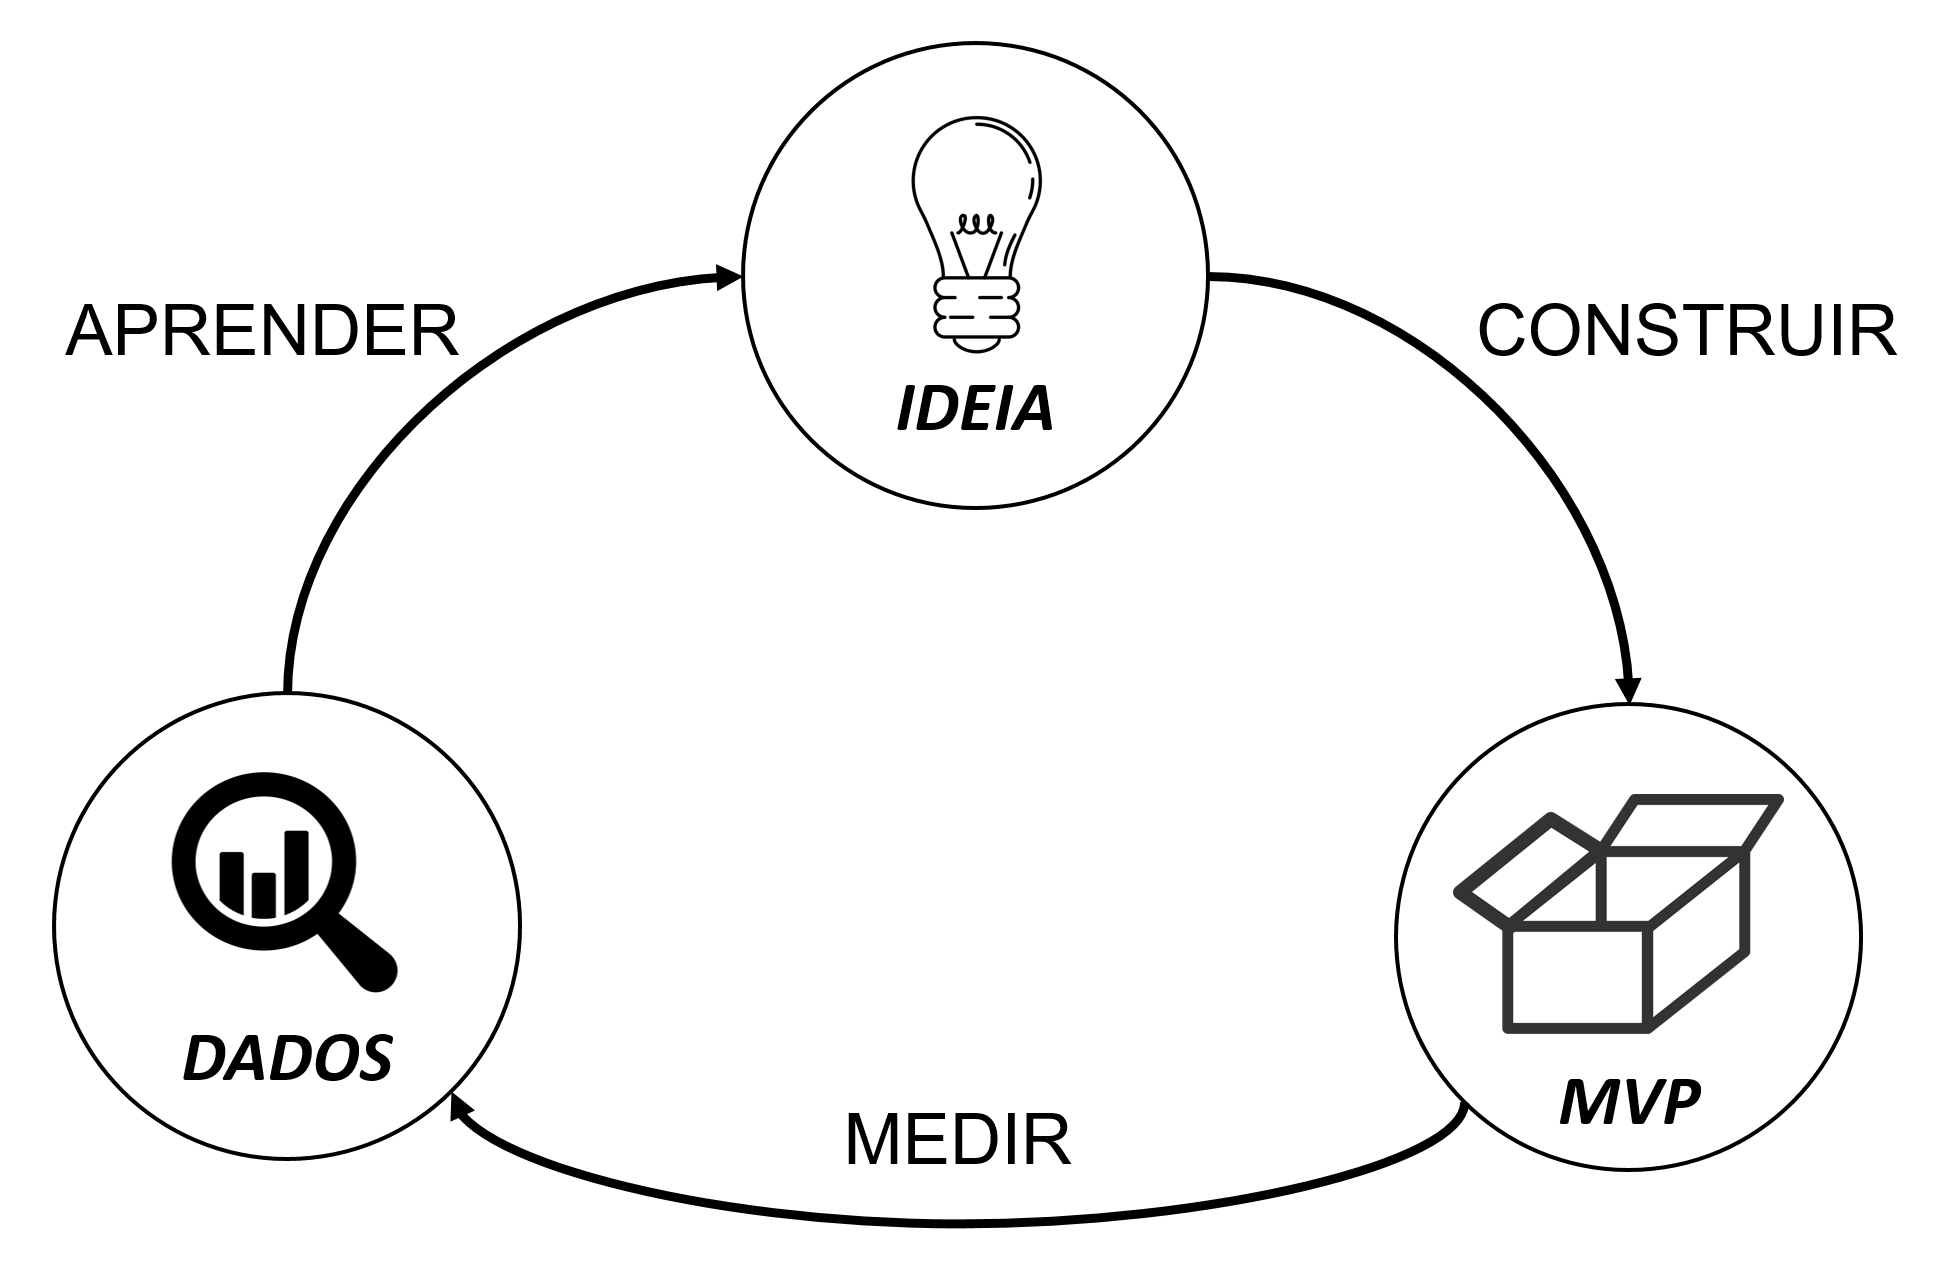
\includegraphics[width=10cm]{images/lean.png}
  		\caption{Lean Startup}
  	\end{center}
  \end{figure}

  Cada ciclo parte de uma ideia na qual o MVP é concebido (CONSTRUIR). Esse produto é colocado no mundo real, para ser validado pelos \textit{stakeholders} (MEDIR). Com o resultado dessas avaliações é necessário identificar, de acordo com a situação, se a próxima etapa será um incremento, pivotamento ou uma nova concepção do zero (APRENDER).
  
  \section{Organização do Trabalho}
  Nos próximos capítulos serão apresentados conceitos, ferramentas e os resultados obtidos com esse trabalho, organizados da seguinte forma:
  
  O capítulo 2 apresentará uma revisão da literatura, trazendo diversos conceitos a respeito de \emph{chatbots}, como seus tipos e também possíveis usos.
  
  O capítulo 3 enumerará uma série de ferramentas, \emph{frameworks} e canais que podem ser utilizados para se construir \emph{chatbots}.
  
  O capítulo 4 apresentará o contexto do projeto PIPA Bot, bem como as escolhas do projeto e suas devidas justificativas, ambientes de desenvolvimento, arquitetura do \emph{chatbot} e as versões do MVP construídas.
  
  O capítulo 5 apresentará a conclusão desse projeto, com o MVP construído no último ciclo de desenvolvimento, limitações encontradas ao longo das etapas e também possíveis melhorias para trabalhos futuros.
 